\section{Applications of Real-Time Object Detection and Multi-Object Tracking}\label{sec:bg-apps}
Real-time object detection and tracking are needed wherever a system must perceive a changing environment continuously and act on what it sees with little delay \cite{li2025motreview,ismail2026realtime}. The same tracking-by-detection pipeline serves very different domains, but the domains differ in the objects of interest, in the camera platform, in the conditions under which the video is recorded, and in how much delay and computation they can accept. This section reviews six major application domains, following the survey published by the author \cite{ismail2026realtime}, and identifies the difficulties that each of them places on detection and tracking. Table~\ref{tab:bg-apps} summarizes them, and Figures~\ref{fig:app-surv}--\ref{fig:app-retail} show a typical system or the main difficulties of each domain. Aerial video from unmanned aerial vehicles, the domain of the experiments of this thesis, is treated in more detail in Section~\ref{sec:bg-app-uav}.

\begin{table}[tbp]
\centering
\caption{Application domains of real-time object detection and multi-object tracking: the objects that are typically tracked, the main difficulties, and the operating constraints.}
\label{tab:bg-apps}
\footnotesize\setlength{\tabcolsep}{4pt}\renewcommand{\arraystretch}{1.25}
\begin{tabular}{>{\raggedright\arraybackslash}p{2.9cm}>{\raggedright\arraybackslash}p{3.2cm}>{\raggedright\arraybackslash}p{4.5cm}>{\raggedright\arraybackslash}p{3.5cm}}
\toprule
Domain & Typical objects & Main difficulties & Operating constraints\\
\midrule
Surveillance and security & people, vehicles, carried objects & crowds, occlusion, day and night lighting, identities across cameras & many continuous streams per server\\
Autonomous vehicles and ADAS & vehicles, pedestrians, cyclists, traffic signs & fast motion, weather and night, safety-critical missed objects & strict latency on the vehicle\\
UAVs and drone tracking & small vehicles and people seen from above & small objects, scale variation, camera motion, occlusion, crowds, changing lighting & onboard or ground-station processing with limited power\\
Industrial robotics & parts, tools, people near the robot & clutter, reflective or textureless parts, precise localization & fixed cycle times, human safety\\
Healthcare and assistive systems & lesions, surgical tools, patients & reliability, false alarms, privacy, scarce annotations & clinical workflows, home monitoring\\
Retail and marketing analytics & customers, products on shelves & dense and similar products, occlusion, privacy & continuous store cameras\\
\bottomrule
\end{tabular}
\end{table}

\subsection{Surveillance and Security}\label{sec:bg-app-surv}
Video surveillance in public spaces, transport hubs, and critical infrastructure is one of the oldest uses of detection and tracking. A detector finds the people and vehicles in each frame, and a tracker keeps their identities so that their paths can be analyzed: a person who enters a restricted area, an object that is left behind, or a vehicle that stops in a prohibited place is recognized from its track rather than from a single frame. Large collections of real surveillance video have also been used to learn to detect anomalous events such as fights, accidents, and robberies \cite{sultani2018anomaly}.

Large sites are covered by many cameras, so tracking is often organized at two levels. Each camera tracks the objects in its own field of view, and a central stage associates the tracks of different cameras with appearance features so that a person keeps one identity across the whole site \cite{ristani2016idf1,ristani2018features}. Figure~\ref{fig:app-surv} shows such a system with four cameras, whose views are matched on a central server by person re-identification. The difficulties of this domain are crowded scenes with frequent occlusion, strong changes of illumination between day and night, and the cost of processing many video streams at the same time, which limits the computation available for each stream.

\begin{figure}[tbp]
\centering
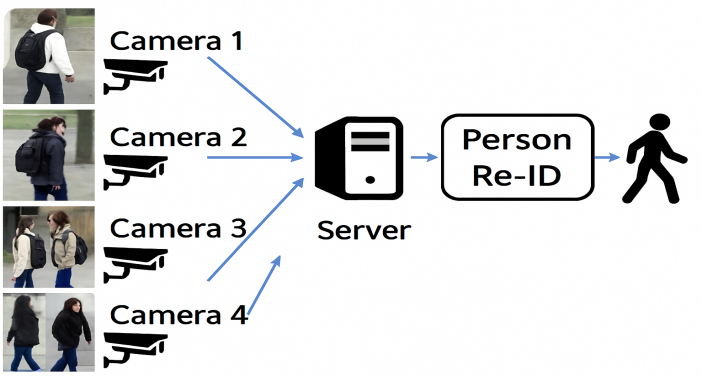
\includegraphics[width=0.85\textwidth]{figures/v4_original/image2.png}
\caption{Multi-camera surveillance system for consistent identity tracking. The views of four cameras are sent to a server, where person re-identification (Re-ID) recognizes the same person in different cameras.}
\label{fig:app-surv}
\end{figure}

\subsection{Autonomous Vehicles and Advanced Driver-Assistance Systems}\label{sec:bg-app-av}
Autonomous vehicles and advanced driver-assistance systems (ADAS) detect and track vehicles, pedestrians, cyclists, and traffic signs around the vehicle. Tracking adds what a single frame cannot provide: the velocity and the recent path of every road user, which are needed to predict its motion and to plan the vehicle's own maneuvers. Public benchmarks recorded from cars, such as KITTI \cite{geiger2012kitti} and nuScenes \cite{caesar2020nuscenes}, provide camera images together with LiDAR and, in nuScenes, radar data. Tracking in this domain is often performed in three dimensions; a simple combination of a Kalman filter and the Hungarian method already gives a strong real-time three-dimensional tracker \cite{weng2020ab3dmot}. Because optical sensors degrade in rain, fog, and snow, the fusion of LiDAR with 4D radar is studied to keep three-dimensional detection reliable in adverse weather \cite{chae2024radar}. Figure~\ref{fig:app-av} shows the processing chain of such a vehicle: high-resolution cameras, LiDAR, and radar are fused, and the fused data are used to detect and track the surrounding objects and to navigate safely. The fusion compensates for the weaknesses of the individual sensors. The main constraints of this domain are a strict latency budget on the vehicle and the safety cost of a missed object. KITTI is also one of the datasets of this thesis (Chapter~\ref{ch:scl}).

\begin{figure}[tbp]
\centering
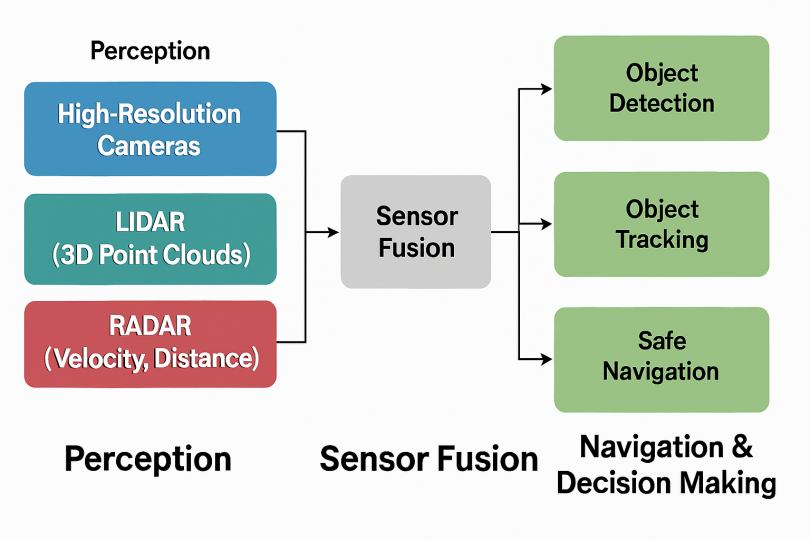
\includegraphics[width=0.80\textwidth]{figures/v4_original/image3.png}
\caption{Multi-modal perception system of an autonomous vehicle based on the fusion of three sensors. High-resolution cameras, LiDAR (three-dimensional point clouds), and radar (velocity and distance) are combined by sensor fusion, which supports object detection, object tracking, and safe navigation.}
\label{fig:app-av}
\end{figure}

\subsection{Unmanned Aerial Vehicles and Drone Tracking}\label{sec:bg-app-uav}
Unmanned aerial vehicles (UAVs) use real-time detection and tracking for traffic monitoring, surveillance, search and rescue, infrastructure inspection, and environmental monitoring \cite{wu2022uavsurvey,kanellakis2017uavvision,bakirci2025lowpower}. The aerospace literature has studied the tracking of multiple ground targets from a multirotor UAV \cite{miller2015multitarget}, feature descriptors for tracking moving ground objects \cite{desai2017uavfeature}, real-time onboard detection of urban objects \cite{lu2024uavdetection}, and vision-based guidance for aerial docking and refueling \cite{choi2022docking,parsons2019refueling}. Two public benchmarks, VisDrone \cite{zhu2022visdrone} and UAVDT \cite{du2018uavdt}, provide annotated drone videos of urban traffic and crowds, and both are used in this thesis. Aerial video combines several difficulties that are less severe in the other domains:
\begin{itemize}
\item \emph{Small objects.} Seen from altitude, a car or a pedestrian may cover only a few pixels. Small objects carry little appearance information and usually receive low detector confidence \cite{cheng2023smallobject,dai2026lsoyolo}.
\item \emph{Scale variation.} The altitude, the viewing angle, and the zoom change the size of the same kind of object within one video and between videos \cite{du2018uavdt,zhu2022visdrone}.
\item \emph{Camera motion.} The platform moves and rotates, so every box shifts between frames even when the objects stand still; the motion model of the tracker must absorb this displacement \cite{liu2022uavmot}.
\item \emph{Occlusion and crowded scenes.} Buildings, trees, bridges, and other vehicles hide objects for some frames, and crowded streets and squares contain many similar objects close together, which makes association and identity preservation difficult \cite{zhu2022visdrone,li2025motreview}.
\item \emph{Variable lighting and weather.} Flights take place by day and at night and under different weather conditions; UAVDT annotates these conditions together with the flying altitude and the camera view \cite{du2018uavdt}.
\item \emph{Real-time processing constraints.} Processing on board, or on a ground station with a limited link, restricts the size of the detector that can run at the frame rate of the video, which is why lightweight detectors are evaluated for drone platforms \cite{bakirci2025lowpower}.
\end{itemize}
Figure~\ref{fig:app-uav} illustrates two of these difficulties, scale variation and camera motion, and the requirements that follow from them: robust feature extraction, data association, and real-time processing. These conditions do not only make aerial tracking difficult; they also change within a single flight. When the scene becomes crowded, the detector passes many weak and false boxes to the tracker; when it becomes sparse or the objects become small, a setting that removed clutter may also remove the few true objects. The quality of the detection stream that reaches the tracker therefore varies over time, and a detector configuration chosen once for the whole video is a compromise over these conditions. In addition, the detector of a UAV system is often replaced by a smaller or compressed model to fit the onboard hardware, which changes the scale of its confidence scores. These two observations motivate the adaptive, training-free control studied in this thesis (Chapters~\ref{ch:acmot} and~\ref{ch:scl}).

\begin{figure}[tbp]
\centering
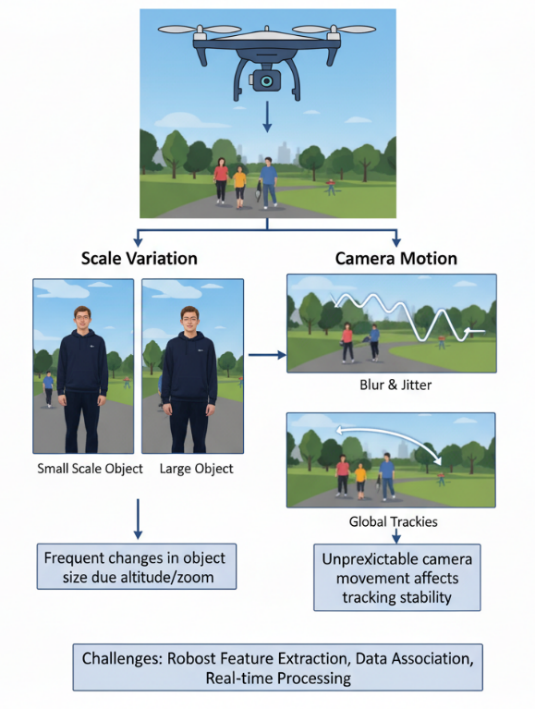
\includegraphics[width=0.70\textwidth]{figures/v4_original/image4.png}
\caption{UAV-based object tracking under scale variation and camera motion. Changes of altitude or zoom change the size of the objects in the image, and the motion of the drone causes blur and jitter; both call for robust feature extraction, data association, and real-time processing.}
\label{fig:app-uav}
\end{figure}

\subsection{Industrial Robotics}\label{sec:bg-app-robot}
In industrial settings, detection and tracking allow robots to locate parts for pick-and-place operations, bin picking, assembly, and quality inspection, and to follow parts that move on conveyors. Learned grasp planning computes robust grasps of objects from depth images \cite{mahler2017dexnet}, and visual simultaneous localization and mapping (SLAM) with ORB features lets a mobile robot estimate its own position from camera images while it moves \cite{murartal2017orbslam2}. Figure~\ref{fig:app-robot} shows a multi-camera tracking system for automated assembly: a local unit detects and tracks the parts in the view of each camera, a central server fuses the local tracks into global identities and trajectories, and these drive the control of the robot and the adjustment of its path in real time. When people work near robots, the detection and tracking of persons also becomes a safety function. The difficulties of this domain are cluttered bins, reflective or textureless parts, the precise localization that manipulation requires, and fixed cycle times.

\begin{figure}[tbp]
\centering
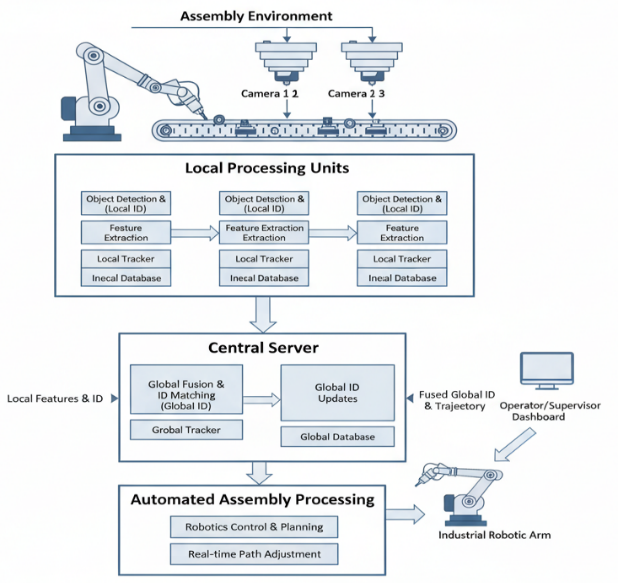
\includegraphics[width=0.95\textwidth]{figures/v4_original/image5.png}
\caption{Industrial robotics system with multi-camera tracking for automated assembly operations. Local processing units detect, describe, and track the parts seen by each camera; a central server matches them into global identities and trajectories, which drive robot control, real-time path adjustment, and an operator dashboard.}
\label{fig:app-robot}
\end{figure}

\subsection{Healthcare and Assistive Systems}\label{sec:bg-app-health}
In medicine, deep detection and segmentation networks localize lesions and anatomical structures in medical images \cite{litjens2017survey}. In surgical video, the presence of instruments and the phases of an operation can be recognized automatically from laparoscopic recordings \cite{twinanda2017endonet}, which supports the monitoring and documentation of procedures. Assistive systems monitor elderly or vulnerable people at home and detect events such as falls with cameras and other sensors \cite{mubashir2013fall}. Figure~\ref{fig:app-health} shows a monitoring system of this kind: wearable and ambient sensors feed a local unit that recognizes activities and detects falls or signs of distress, alerts reach clinicians and caregivers, and a central server keeps the records and analyzes them over time. This domain requires high reliability and few false alarms, must respect the privacy of patients, and often has only small annotated datasets.

\begin{figure}[tbp]
\centering
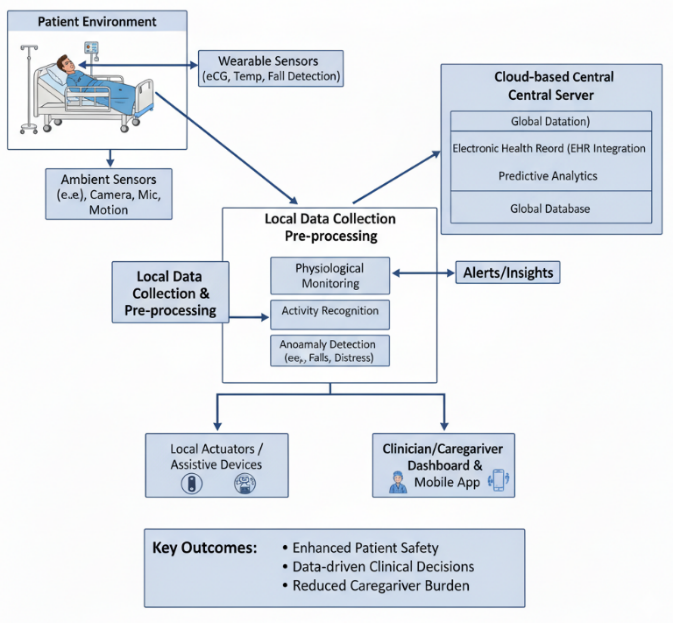
\includegraphics[width=0.95\textwidth]{figures/v4_original/image6.png}
\caption{Healthcare monitoring system for patient safety and assistive care. Wearable and ambient sensors feed a local unit for physiological monitoring, activity recognition, and anomaly detection (falls, distress), which issues alerts, drives assistive devices and caregiver dashboards, and exchanges data with a cloud server for health records and predictive analytics.}
\label{fig:app-health}
\end{figure}

\subsection{Retail and Marketing Analytics}\label{sec:bg-app-retail}
In retail, detection and tracking are used to count customers, to measure how they move through a store and how long they stay in front of displays, and to monitor shelves for missing or misplaced products. Shelf images contain many small, similar, and tightly packed products, which are hard to separate with standard detectors \cite{goldman2019dense}, and product recognition must handle thousands of classes with similar packaging that change frequently \cite{wei2020retail}. Automated checkout systems combine the tracking of customers with the recognition of the products they pick up. Figure~\ref{fig:app-retail} shows a system of this kind, in which the same local tracking serves both automated checkout and the analytics of the store. Occlusion by other customers and the protection of customers' privacy are the main practical concerns.

\begin{figure}[tbp]
\centering
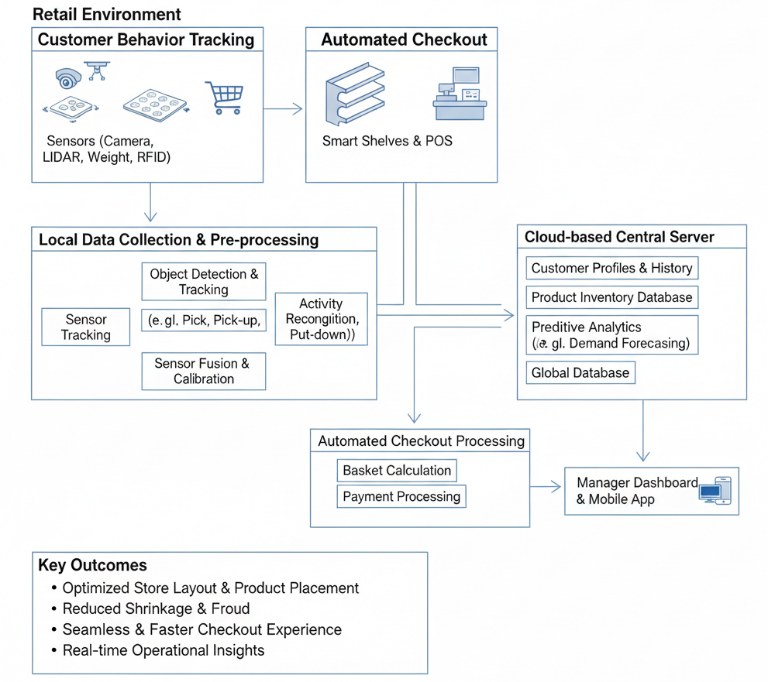
\includegraphics[width=0.90\textwidth]{figures/v4_original/image7.png}
\caption{Retail analytics system for customer tracking and automated checkout. Store sensors feed a local unit for object detection and tracking, activity recognition, and sensor fusion; its results drive automated checkout and a cloud server for customer profiles, inventory, and predictive analytics, with a manager dashboard.}
\label{fig:app-retail}
\end{figure}

\emph{From applications to technical requirements.} Across these domains, the same pipeline is asked to detect the objects of interest reliably, to keep their identities over time, and to do so within the delay and the computation that the platform allows. The domains differ in which of these demands is the hardest, and aerial video combines several of them: small and crowded objects, a moving camera, changing conditions, and limited onboard computation. The next section introduces the technical background needed to address these demands: how detectors produce boxes and scores, how trackers use them, how the scores are read through thresholds, and how tracking accuracy is measured.
